\scanpage{78}
\mspage{38}
Soit donc $\underline G'$ un MD-graphe quotient de $\underline G$ -- par un ens. \inserted{$C$} d'arêtes du graphe $G$ sous-jacent à $\underline G$,
\[
(96)\qquad\underline G'=\underline G/C.
\]
On a alors un \inserted{diagramme de} morphismes canoniques
\diagram{\begin{tikzpicture}[x=1cm,y=1cm]
\node at (-3.1,.85) {$(97)$};
\node at (0,1.8) {$\overset{\deleted{\unsure{\wedge}}}{M}_{\underline G}$};
\node at (3.0,1.9) {$\deleted{\unsure{\widehat M_{\underline G'}}}$};
\node at (0,0) {$\widehat M_{\underline G}$};
\node at (3.0,.12) {$\widehat M_{\underline G'}$};
\node at (1.48,1.80) {$\deleted{\longrightarrow}$};
\draw (.10,1.11) .. controls (.25,1.28) and (-.13,1.36) .. (-.13,1.10)
 -- (.02,.56);
\draw (3.12,1.24) .. controls (3.24,1.40) and (2.85,1.46) .. (2.87,1.20)
 -- (3.00,.65);
\draw (2.86,.82)--(3.00,.65)--(3.15,.84);
\draw (2.59,1.34)--(3.48,1.78)--(2.62,1.05)--(3.48,1.46)
 --(2.64,.73)--(3.46,1.12)--(2.70,.48);
\draw[->] (.86,.05)--(2.18,.10);
\end{tikzpicture}}
\margin{déployer la déf. de $\Gamma^!_{\underline G,\underline G'}$ !}
Si on désigne par $\Gamma^!_{\underline G,C}$ ou $\Gamma^!_{\underline G,\underline G'}$ le sous-groupe de $\Gamma_{\underline G}$ qui est formé des autom qui transforment $C$ en lui-$=$, et qui induisent l'identité sur $\underline G'$, \unsure{la flèche|l'hom.} \deleted{\unsure{verticale}} \inserted{horizontale} $\underset{\unsure{
\begin{tikzpicture}[baseline=-.5ex,x=.10cm,y=.10cm]
\draw[line width=.4pt] (0,1)--(.8,2.3)--(1.3,2.5)--(1.0,.45)
 .. controls (.75,-.1) and (1.5,-.1) .. (1.9,.3)--(2.3,.15)--(1.7,.75);
\draw[line width=.4pt] (0,1)--(1.28,1.17)--(.70,.28)--(.38,.45)--(.82,2.30);
\end{tikzpicture}}}{\text{de}}$ (97) se factorise \deleted{\unsure{donc}} \inserted{une} immersion de multiplicités
\diagram{(98):\qquad\begin{tikzcd}[ampersand replacement=\&]
(\widehat M_{\underline G},\Gamma^!_{\underline G,\underline G'})\arrow[r,hook] \& \widehat M_{\underline G'}
\end{tikzcd}}
\margin{Ce ne sont peut-être que des immersions \uline{locales}, il me semble -- à vérifier\ldots}
Je désigne par $\widehat M_{\underline G,\underline G'}$ le \uline{germe de multiplicité} défini par l'inclusion (98), et par $M_{\underline G,\underline G'}$ le germe défini par l'inclusion induite
\diagram{(99)\qquad\begin{tikzcd}[ampersand replacement=\&]
(M_{\underline G},\Gamma^!_{G,G'})\arrow[r,hook] \& \widehat M_{\underline G'}
\end{tikzcd}}
\margin{Il vaut mieux considérer le germe de multiplicité défini par l'\uline{immersion locale} $M_{\underline G}\longrightarrow\unsure{M_{\underline G'}|\widehat M_{\underline G'}}$, et faire opérer $\Gamma^{\unsure{!}}_{\underline G,G'}$ dessus, \unsure{et ce sera} $M_{\underline G,\underline G'}$}
\margin{77}
